\begin{frame}{Relevant Questions}
    \textbf{RQ4: How explainable are the evaluation ratings of {\llm}s?}
    \begin{itemize}
        \item How specific to the given criteria are the explanations provided by LLMs?
        \item What sort of issues do LLM explanations display?
        \item How well can LLMs be thought to understand the ASE task?
        \item Can studying LLM pretraining data help explain their ASG performance?
    \end{itemize}
\end{frame}

\begin{frame}{Clustering of Explanation Embeddings}
    \begin{figure}[h!]
        \centering
        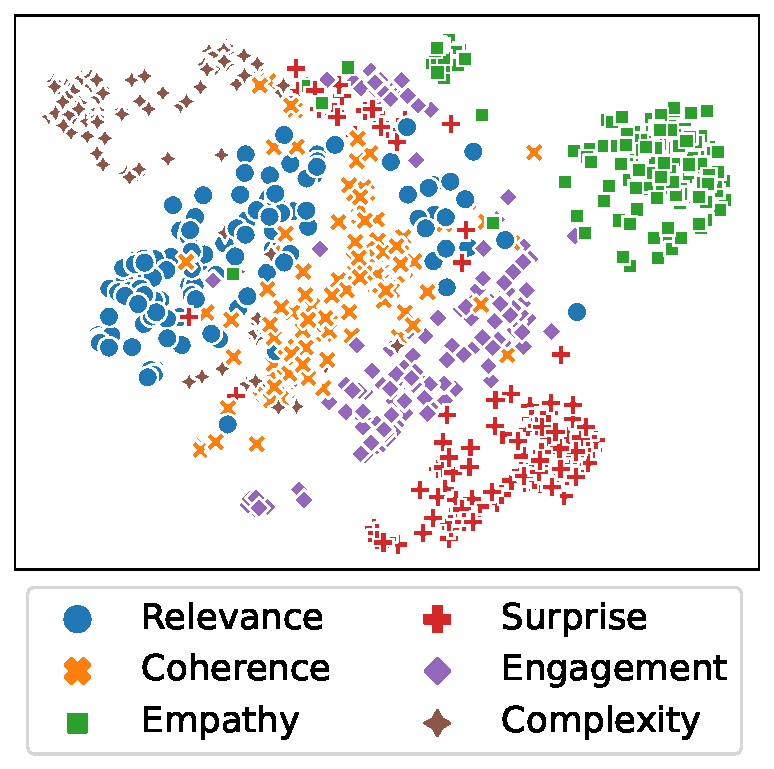
\includegraphics[width=0.45\columnwidth]{pictures/embedding_umap_beluga.pdf}
        \caption{UMAP projection of Beluga-13B explanations.}
        \label{fig:umap_explanation_beluga}
    \end{figure}
    \vspace*{-0.4cm}
    LLM explanations are overall well-separated \wrt\ their corresponding criteria.
\end{frame}

\begin{frame}{Keyword Analysis}
    \begin{table}[!h]
        \scriptsize
        \centering
        \begin{tabular}{cp{0.85\linewidth}}
        \toprule
        \textbf{Crit.} & \textbf{Keywords}\\
        \midrule
        RE & story, prompt, roughly matches, target, weak relationship, connection, weak, focuses, unrelated, human story provided, idea, difficult, writing\\
        \midrule
        CH & story, coherence, make sense, difficult to understand, clear narrative structure, follow, making it difficult, rate, context, jumps, understandable plot\\
        \midrule
        EM & empathy, emotions, understand the characters, depth, emotional connection, clear, feelings, context, fully, level, specific, thoughts, sadness, recognize\\
        \midrule
        SU & story, surprise, ending, predictable, rate, unexpected, twist, completely obvious, human, plot, abruptly, resolution, half, context, offer, hints\\
        \midrule
        EG & story, mildly interesting, engagement, difficult, found, characters, fully engage, clear plot, clear narrative, unique, felt disjointed, protagonist\\
        \midrule
        CX &  story, characters, intricate plot, difficult to understand, straightforward, depth, simple, extremely simple, involves, development, details\\
        \bottomrule
        \end{tabular}
        \caption{Selected keywords from Beluga-13B explanations w.r.t.\ a specific criterion. Keywords are semantically relevant to the criterion.}
        \label{tab:explanation_keywords}
    \end{table}
\end{frame}

\begin{frame}{User Study on LLM Explanations}
    We ask human raters to identify issues in 100 randomly sampled LLM Eval-Prompt 3 explanations. We distinguish 5 error categories:
    \begin{enumerate}
        \item \textbf{Poor Syntax}: parts of the explanation are grammatically incorrect or wrongly-worded;
        \item \textbf{Incoherence}: parts of the explanation are self-contradictory, logically wrong, or simply do not make sense and do not fit the other categories;
        \item \textbf{Wrong Guideline}: the explanation is not faithful to the predicted rating according to the provided guidelines;
        \item \textbf{Superfluous Text}: parts of the explanation contain text that repeats itself or generation artefacts;
        \item \textbf{Unsubstantiated Claims}: the explanation fails to make explicit references to the story to substantiate its reasoning.
    \end{enumerate}
\end{frame}

\begin{frame}{User Study on LLM Explanations}
    \begin{table}[!h]
        \centering
        \begin{tabular}{lcc}
        \toprule
        \textbf{Error Type} & \textbf{Rate} & \textbf{AC1} \\
        \midrule
        No Explanation* & 0.40 & --- \\
        \midrule
        Poor Syntax & 0.02 & \resultscr{0.97}{0.03}\\
        Incoherence & 0.11 & \resultscr{0.81}{0.08}\\
        Wrong Guideline & 0.13 & \resultscr{0.90}{0.06}\\
        Superfluous Text & 0.20 & \resultscr{0.66}{0.12}\\
        Unsubstantiated Claims & 0.31 & \resultscr{0.60}{0.14}\\
        \bottomrule
        \end{tabular}
        \caption{Error rates of Beluga-13B Eval-Prompt 3 on a sample of 100 explanations. Lower is better. The asterisk signals that all 1,056 Eval-Prompt 3 annotations were considered.}
        \label{tab:error_rates}
    \end{table} 
    \vspace*{-0.4cm}
    High rate of ``Unsubstantiated Claims'', and \textbf{40\% of all Eval-Prompt 3 ratings did not even have an explanation}.
\end{frame}

\begin{frame}{Influence of Pretraining Data}
    \begin{itemize}
        \item We use the \minkprob\ detection method \citep{shi2023detecting}, based on the hypothesis that unseen data will contain more outlier words with low probability than seen data. 
        \item We showed that \textbf{it is easier to detect if a book was in the training data of a larger LLM}, and that larger LLMs tend to produce text that is \textbf{more faithful to their training data}.
        \item $\hookrightarrow$ This could explain the better ASG performance of larger {\llm}s.
    \end{itemize}
\end{frame}

\begin{frame}{Summary}
    \textbf{RQ4: How explainable are the evaluation ratings of {\llm}s?}
    \begin{itemize}
        \item We performed different experiments, including a user study on LLM explanations and an estimation of the influence of pretraining data on LLM performance;
        \item \textbf{LLMs understand the ASE task only partially:} while they provide explanations that are specific to the evaluated criteria, they struggle to explain their answers with substantiated claims;
        \item \textbf{Pretraining data helps explain LLM performance at ASG:} the higher ratings of larger LLMs may be due to their ability to produce output similar to existing books.
    \end{itemize}
\end{frame}